\documentclass[tikz,border=2pt]{standalone}
\usepackage{amsmath,amssymb}
\usepackage{tikz}
\usetikzlibrary{arrows.meta}

\begin{document}
% An outcome is a single element of the sample space: this roll produced omega = 4.
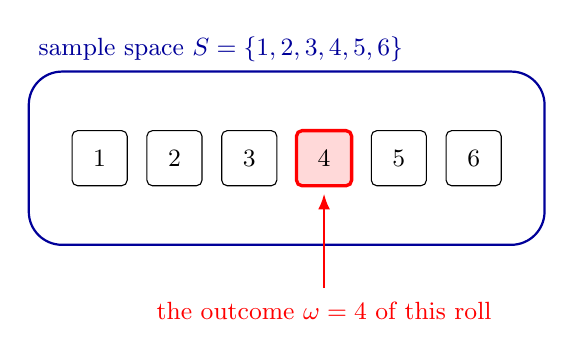
\begin{tikzpicture}[every node/.style={font=\small}, >={Latex[length=2mm]}]
	\draw[thick, blue!60!black, rounded corners=12pt] (-0.4,0.1) rectangle (6.15,2.3);
	\node[blue!60!black, anchor=south west] at (-0.4,2.3) {sample space $S=\{1,2,3,4,5,6\}$};
	\foreach \i in {1,...,6} {
		\pgfmathsetmacro{\x}{0.5+(\i-1)*0.95}
		\node[draw, fill=white, rounded corners=2pt, minimum size=7mm] at (\x,1.2) {$\i$};
	}
	\node[draw=red, very thick, fill=red!15, rounded corners=2pt, minimum size=7mm] at (3.35,1.2) {$4$};
	\draw[->, red, thick] (3.35,-0.45) -- (3.35,0.75);
	\node[red, anchor=north] at (3.35,-0.5) {the outcome $\omega=4$ of this roll};
	
\end{tikzpicture}
\end{document}
